%%%%%%%%%%%%%%%%%%%%%%%%%%%%%%%%%%%%%%%%%
% Wenneker Article
% LaTeX Template
% Version 2.0 (28/2/17)
%
% This template was downloaded from:
% http://www.LaTeXTemplates.com
%
% Authors:
% Vel (vel@LaTeXTemplates.com)
% Frits Wenneker
%
% License:
% CC BY-NC-SA 3.0 (http://creativecommons.org/licenses/by-nc-sa/3.0/)
%
%%%%%%%%%%%%%%%%%%%%%%%%%%%%%%%%%%%%%%%%%

%----------------------------------------------------------------------------------------
%	PACKAGES AND OTHER DOCUMENT CONFIGURATIONS
%----------------------------------------------------------------------------------------

\documentclass[10pt, a4paper, twocolumn]{article} % 10pt font size (11 and 12 also possible), A4 paper (letterpaper for US letter) and two column layout (remove for one column)

%%%%%%%%%%%%%%%%%%%%%%%%%%%%%%%%%%%%%%%%%
% Wenneker Article
% Structure Specification File
% Version 1.0 (28/2/17)
%
% This file originates from:
% http://www.LaTeXTemplates.com
%
% Authors:
% Frits Wenneker
% Vel (vel@LaTeXTemplates.com)
%
% License:
% CC BY-NC-SA 3.0 (http://creativecommons.org/licenses/by-nc-sa/3.0/)
%
%%%%%%%%%%%%%%%%%%%%%%%%%%%%%%%%%%%%%%%%%

%----------------------------------------------------------------------------------------
%	PACKAGES AND OTHER DOCUMENT CONFIGURATIONS
%----------------------------------------------------------------------------------------

\usepackage[english]{babel} % English language hyphenation

\usepackage{microtype} % Better typography

\usepackage{amsmath,amsfonts,amsthm} % Math packages for equations

\usepackage[svgnames]{xcolor} % Enabling colors by their 'svgnames'

\usepackage[hang, small, labelfont=bf, up, textfont=it]{caption} % Custom captions under/above tables and figures

\usepackage{booktabs} % Horizontal rules in tables

\usepackage{lastpage} % Used to determine the number of pages in the document (for "Page X of Total")

\usepackage{graphicx} % Required for adding images

\usepackage{enumitem} % Required for customising lists
\setlist{noitemsep} % Remove spacing between bullet/numbered list elements

\usepackage{sectsty} % Enables custom section titles
\allsectionsfont{\usefont{OT1}{phv}{b}{n}} % Change the font of all section commands (Helvetica)

%----------------------------------------------------------------------------------------
%	MARGINS AND SPACING
%----------------------------------------------------------------------------------------

\usepackage{geometry} % Required for adjusting page dimensions

\geometry{
	top=1cm, % Top margin
	bottom=1.5cm, % Bottom margin
	left=2cm, % Left margin
	right=2cm, % Right margin
	includehead, % Include space for a header
	includefoot, % Include space for a footer
	%showframe, % Uncomment to show how the type block is set on the page
}

\setlength{\columnsep}{7mm} % Column separation width

%----------------------------------------------------------------------------------------
%	FONTS
%----------------------------------------------------------------------------------------

\usepackage[T1]{fontenc} % Output font encoding for international characters
\usepackage[utf8]{inputenc} % Required for inputting international characters

\usepackage{XCharter} % Use the XCharter font

%----------------------------------------------------------------------------------------
%	HEADERS AND FOOTERS
%----------------------------------------------------------------------------------------

\usepackage{fancyhdr} % Needed to define custom headers/footers
\pagestyle{fancy} % Enables the custom headers/footers

\renewcommand{\headrulewidth}{0.0pt} % No header rule
\renewcommand{\footrulewidth}{0.4pt} % Thin footer rule

\renewcommand{\sectionmark}[1]{\markboth{#1}{}} % Removes the section number from the header when \leftmark is used

%\nouppercase\leftmark % Add this to one of the lines below if you want a section title in the header/footer

% Headers
\lhead{} % Left header
\chead{\textit{\thetitle}} % Center header - currently printing the article title
\rhead{} % Right header

% Footers
\lfoot{} % Left footer
\cfoot{} % Center footer
\rfoot{\footnotesize Page \thepage\ of \pageref{LastPage}} % Right footer, "Page 1 of 2"

\fancypagestyle{firstpage}{ % Page style for the first page with the title
	\fancyhf{}
	\renewcommand{\footrulewidth}{0pt} % Suppress footer rule
}

%----------------------------------------------------------------------------------------
%	TITLE SECTION
%----------------------------------------------------------------------------------------

\newcommand{\authorstyle}[1]{{\large\usefont{OT1}{phv}{b}{n}\color{DarkRed}#1}} % Authors style (Helvetica)

\newcommand{\institution}[1]{{\footnotesize\usefont{OT1}{phv}{m}{sl}\color{Black}#1}} % Institutions style (Helvetica)

\usepackage{titling} % Allows custom title configuration

\newcommand{\HorRule}{\color{DarkGoldenrod}\rule{\linewidth}{1pt}} % Defines the gold horizontal rule around the title

\pretitle{
	\vspace{-30pt} % Move the entire title section up
	\HorRule\vspace{10pt} % Horizontal rule before the title
	\fontsize{32}{36}\usefont{OT1}{phv}{b}{n}\selectfont % Helvetica
	\color{DarkRed} % Text colour for the title and author(s)
}

\posttitle{\par\vskip 15pt} % Whitespace under the title

\preauthor{} % Anything that will appear before \author is printed

\postauthor{ % Anything that will appear after \author is printed
	\vspace{10pt} % Space before the rule
	\par\HorRule % Horizontal rule after the title
	\vspace{20pt} % Space after the title section
}

%----------------------------------------------------------------------------------------
%	ABSTRACT
%----------------------------------------------------------------------------------------

\usepackage{lettrine} % Package to accentuate the first letter of the text (lettrine)
\usepackage{fix-cm}	% Fixes the height of the lettrine

\newcommand{\initial}[1]{ % Defines the command and style for the lettrine
	\lettrine[lines=3,findent=4pt,nindent=0pt]{% Lettrine takes up 3 lines, the text to the right of it is indented 4pt and further indenting of lines 2+ is stopped
		\color{DarkGoldenrod}% Lettrine colour
		{#1}% The letter
	}{}%
}

\usepackage{xstring} % Required for string manipulation

\newcommand{\lettrineabstract}[1]{
	\StrLeft{#1}{1}[\firstletter] % Capture the first letter of the abstract for the lettrine
	\initial{\firstletter}\textbf{\StrGobbleLeft{#1}{1}} % Print the abstract with the first letter as a lettrine and the rest in bold
}

%----------------------------------------------------------------------------------------
%	BIBLIOGRAPHY
%----------------------------------------------------------------------------------------

\usepackage[backend=bibtex,style=authoryear,natbib=true, sorting=none]{biblatex} % Use the bibtex backend with the authoryear citation style (which resembles APA)

\addbibresource{example.bib} % The filename of the bibliography

\usepackage[autostyle=true]{csquotes} % Required to generate language-dependent quotes in the bibliography
 % Specifies the document structure and loads requires packages
\usepackage[font=small,labelfont=bf,margin=\parindent,tableposition=top]{caption}
\usepackage{float}
\usepackage{blindtext}

%----------------------------------------------------------------------------------------
%	ARTICLE INFORMATION
%----------------------------------------------------------------------------------------

\title{Methylation Analysis of DepMap Data} % The article title

\author{
	\authorstyle{Ashir Borah\textsuperscript{1}} % Authors
	\newline\newline % Space before institutions
	\textsuperscript{1}\institution{BMI PhD Program, University of California, San Francisco}\\ % Institution 1
}

% Example of a one line author/institution relationship
%\author{\newauthor{John Marston} \newinstitution{Universidad Nacional Autónoma de México, Mexico City, Mexico}}

\date{\today} % Add a date here if you would like one to appear underneath the title block, use \today for the current date, leave empty for no date

%----------------------------------------------------------------------------------------

\begin{document}

\maketitle % Print the title

\thispagestyle{firstpage} % Apply the page style for the first page (no headers and footers)

%----------------------------------------------------------------------------------------
%	ABSTRACT
%----------------------------------------------------------------------------------------

\lettrineabstract{Methylation impacts the epigenomic state of cells and has been implicated in cancer. Epigenomic changes can impact cancer cell line viability, presenting new cancer targets. Downstream analysis of probe-level data is challenging to arrive at a biological hypothesis. GOMeth  helps discover new targets previously not possible, presenting new avenues for cancer therapeutics development  }

%----------------------------------------------------------------------------------------
%	ARTICLE CONTENTS
%----------------------------------------------------------------------------------------

\section{Problem statement}

The Dependency Map project has performed genome-scale CRISPR knockout in cancer cell lines \citep{Tsherniak2017-mc}. This data presents an incredible resource for new therapeutic discovery if an observed clinically exploitable phenotype can be tied to molecular features. While such analysis has been performed for different data types like RNAseq, Mutation, Fusion, Metabolomics and Proteomics \citep{Dempster2020.02.21.959627}, a systematic Methylation analysis is missing. DepMap stopped producing Infinium 450k Methylation array data after a few cycles. 

A large Methylation dataset for cancer cell lines \citep{Iorio2016-mq} presents an opportunity to model the cancer cell lines data using Methylation data. Models with high predictive performance need further analysis to build confidence before further validation in the lab. GOMeth \citep{Maksimovic2021} can help link probes predictive to a biological process.

The methylation data has 450,000 probes, each enabling the measurement of the methylation levels at these CpG sites. These measurements, along with other informative features like the lineage of the cell lines and confounders, are used to model the observed viability data after knockout.


%------------------------------------------------

\section{Results}

Methylation data has a wide degree of predictive power based on the knockout being studied. Knockout of lineage-specific essential genes like SOX10 for skin lineages are not interesting targets, and they are easily spotted with a lineage feature having very high feature importance. 

\begin{figure*}
	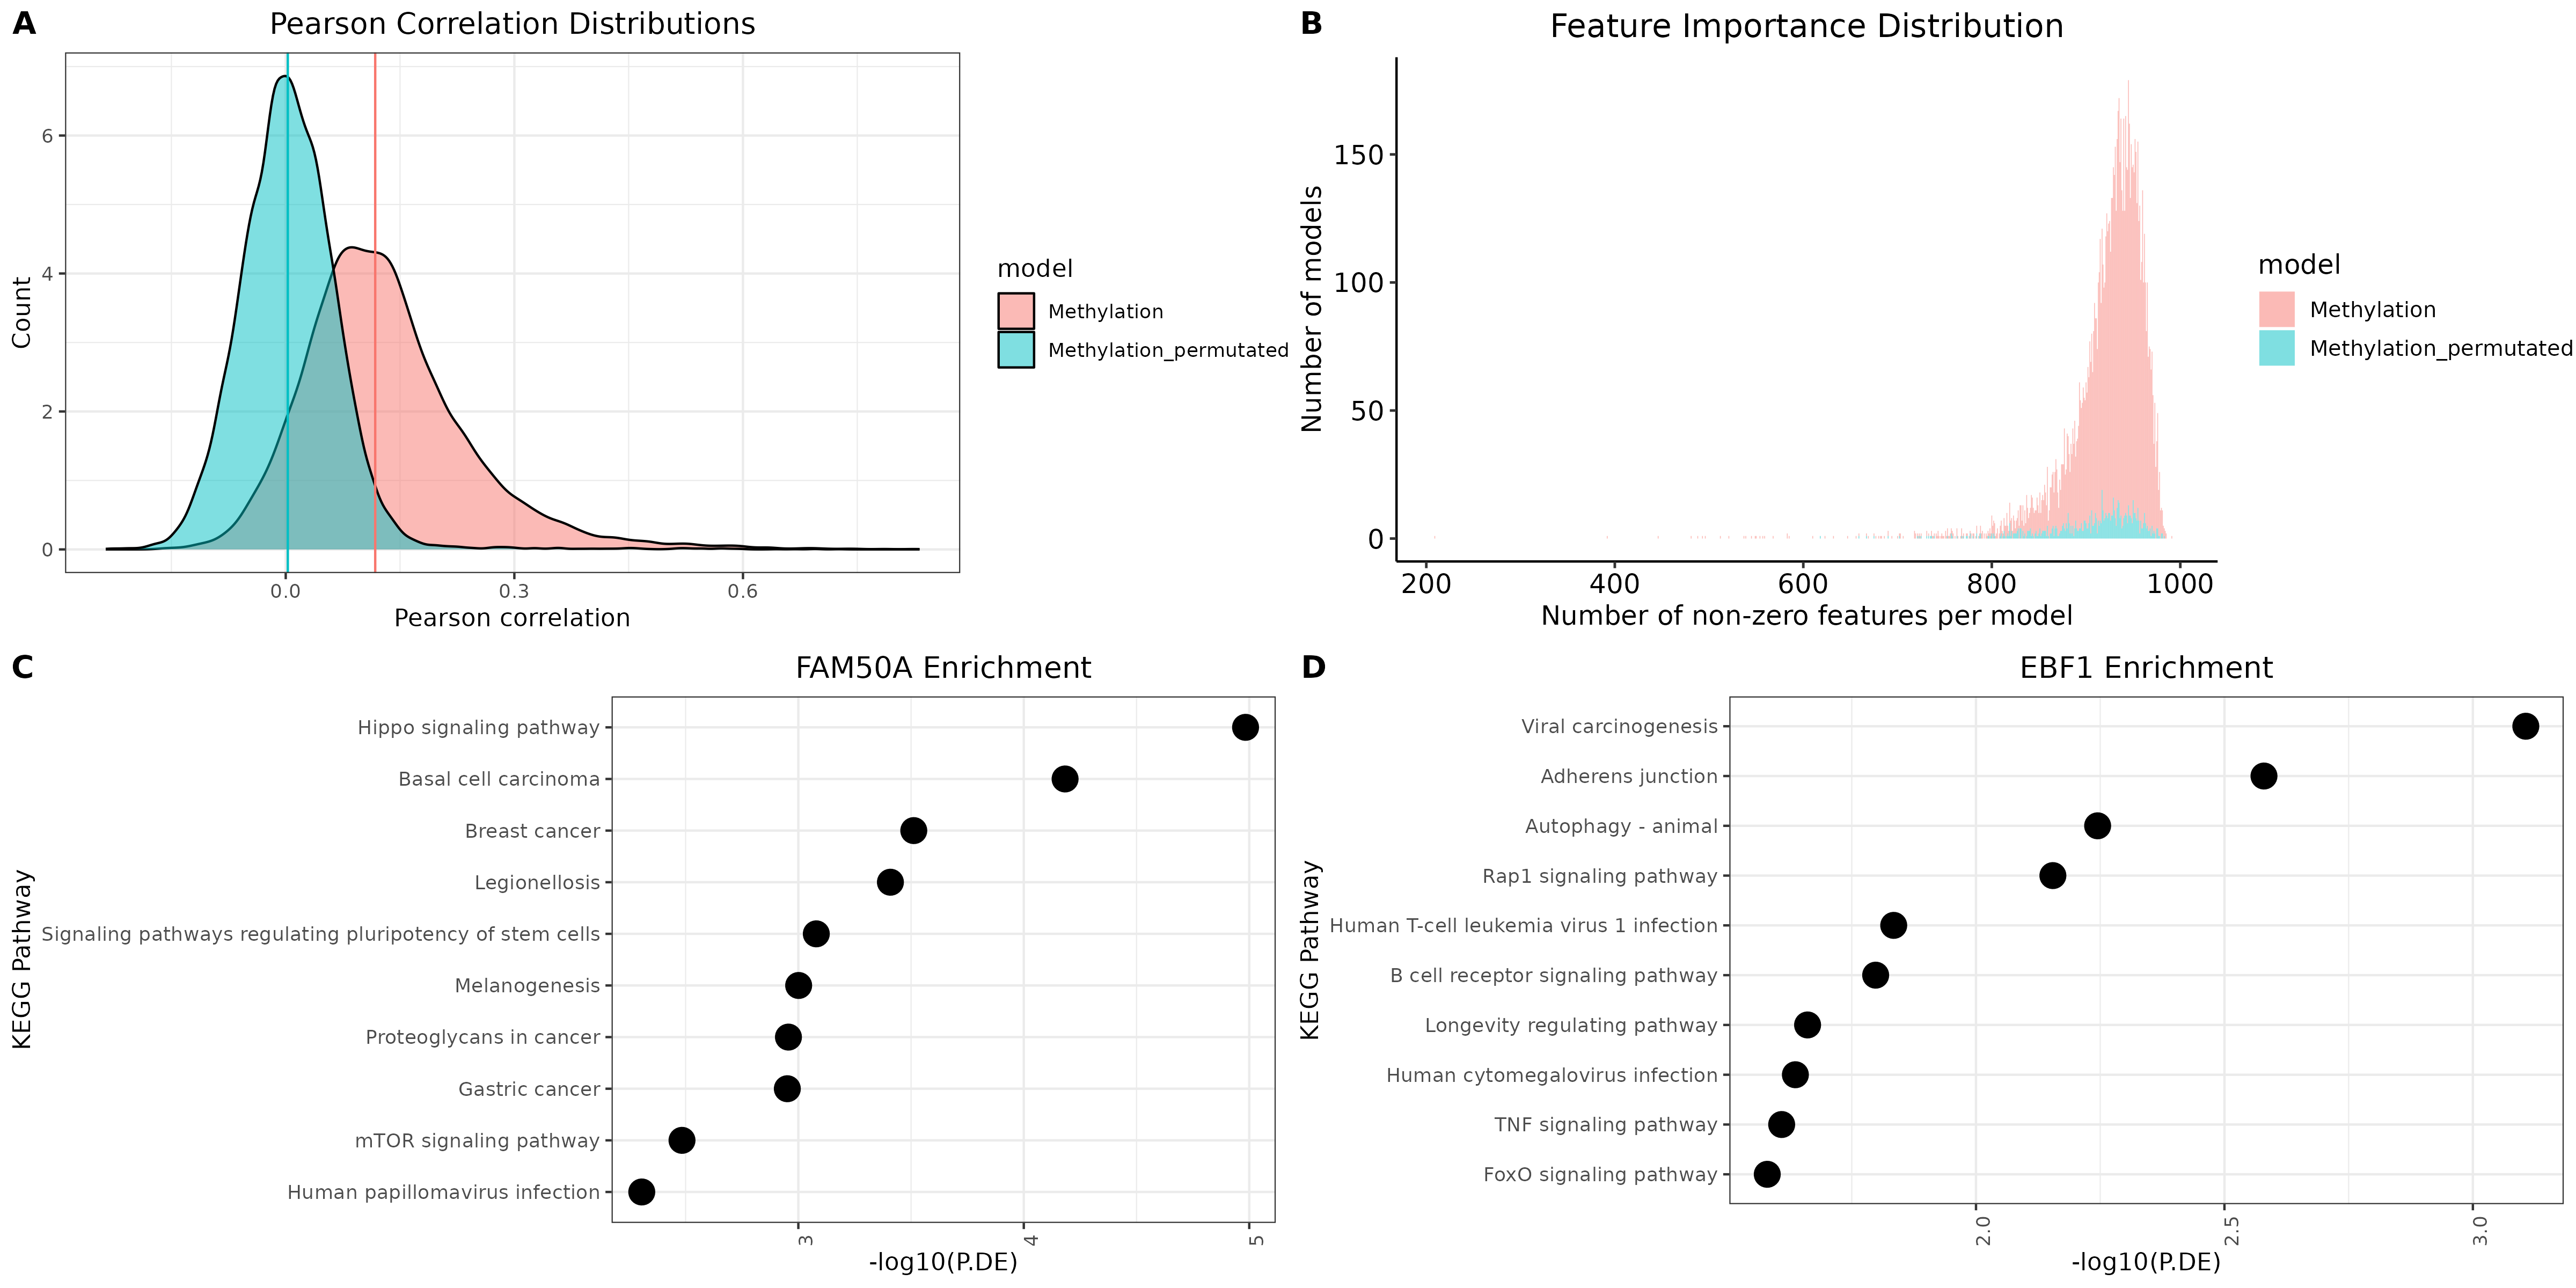
\includegraphics[width=\textwidth]{summary.png} % Figure image
	\caption{Methylation Analysis of DepMap Data} % Figure caption
    \caption*{(A) Pearson correlation distribution between the observed and predicted values. The blue line represents the }
	\label{pearson} % Label for referencing with \ref{bear}
\end{figure*}

As shown in Figure \ref{pearson}A, the Pearson correlation of the methylation data is shifted to the right of the permuted methylation data indicating that the methylation data improved predictive performance overall. The medians of the distributions in Table \ref{model_performance} reflect this fact. When the feature importance of the statistically significant models are analysed using GOMeth (details in Methods), cancer pathways are seen to be enriched in the probes that were predictive of cell viability data.

Some of the top models are already implicated in cancer(EBF1 \citep{Shen2020-gq}, FAM50A \citep{KOFERLE2022110636}). Further analysis with biological experts might reveal new theraputics targets for cancer.


\begin{table}
	\caption{Model performance}
	\centering
	\begin{tabular}{llr}
		\toprule
		\cmidrule(r){1-2}
		Model & Mean $\rho$ \\
		\midrule
		Methylation & $0.132$  \\ 
		Methylation-permutated & $0.00491$ \\
		\bottomrule
            \label{model_performance}
	\end{tabular}
\end{table}



\section{Methods}

\subsection{Modeling}
Methylation data from \citep{Iorio2016-mq} is processed with the SeSAMe  \citep{10.1093/nar/gky691} to replicate the processing of TCGA to make values comparable. The other datasets used from modeling was downloaded from \citep{DepMap2022}.

Features:

\begin{itemize}
    \item Infinium 450k Methylation beta values
    \item One hot encoded lineage
    \item Confounders
\end{itemize}

The predicted viability dataset is the Chronos CRISPR gene effects dataset \citep{DepMap2022, Dempster2021}. A random forest regression model from \citep{Krill-Burger2022.03.02.482624} was used to predict the gene effect data. To evaluate the effect of adding the Methylation data and differentiate the boost in performance merely from adding additional features, the methylation dataset was permutated while keeping other features like lineage and confounders unchanged. 

Feature importances from these random forest models were extracted to further analyze the predictions. The feature importance from the permutated models were used to generate a null distribution enabling the calculation of p-values. This feature importance was used as a cut off for enrichment analysis using GOMeth \citep{Maksimovic2021}.

\subsection{Analysis of models}

\section{Discussions}


\section{Conclusions}





%----------------------------------------------------------------------------------------
%	BIBLIOGRAPHY
%----------------------------------------------------------------------------------------
\clearpage
\printbibliography[title={Bibliography}] % Print the bibliography, section title in curly brackets

%----------------------------------------------------------------------------------------

\end{document}
